To validate the optimization script, several test cases have been done.
% Diversi aspetti del problema si sono dovuti testare, al fine di ottenere informazioni sull' effettivo funzionamento del programma, nonchè al fine di far emergere errori e complicazioni non tenute in conto in fase di programmazione. Si sono quindi effettuati test su diversi modelli di ala, in particolare l' ala di Goland e la CRW della NASA, caratterizzati da un livello di dettaglio delle mesh strutturali diversi, noanchè da proprietà aerodinamiche diverse. Inoltre nei vari test si sono usati entrambi i driver scelti per l' implementazione, COBYLA e SLSQP, con i corrispettivi confronti sui risultati; e diverse combinazioni tra objective function and constraints si sono effettutate. 
Many aspects of the problem had to be tested, in order to obtain information on the effective functioning of the software, as well as to bring out errors and complications not taken into account in the programming phase. Tests were therefore carried out on different wing models, in particular the Goland wing and the NASA Common Research Wing CRM , characterized by a different  level of detail of the structural meshes, as well as by different aerodynamic properties. Moreover, in the various tests both drivers chosen for the implementation, COBYLA and SLSQP, were used, with the corresponding comparisons on the results; and different combinations between objective function and constraints were carried out. \\
As first let's see in details the wing model used for the validation of the software.
\section{Goland Wing}
The Goland wing is a wing model developed by M. Goland, and described in \cite{gola}. This model of wing is really simple, and several numerical and experimental studies have been carried out on this wing, which is usually used as reference to validate aeroelastic codes. So for the preliminary approach it's the best choice, because we can obtain fast results and find in literature many works to compare the results.\\
The Goland wing model that we use is based on the model described in the work of Beran P.S. \cite{bera}\\
The wing is schematized as a cantilevered wing. The wing span is 6.10 m, the chord 1.22 m and the thickness 0.51 m.\\
The finite element model is built up from shear panels, modeling the spars and ribs, and membrane elements, modeling the wing skins. The spar and rib caps are modeled by rod elements and posts connect the wing skins at every spar/rib intersection.\cite{sito} In Fig. \ref{fig:5_1} is showed how the initial FEM model is structured.\\
The result is a very flexible wing, that it's ideal to show several aeroelastic behavior.\\
\begin{figure}[H]
	\centering
	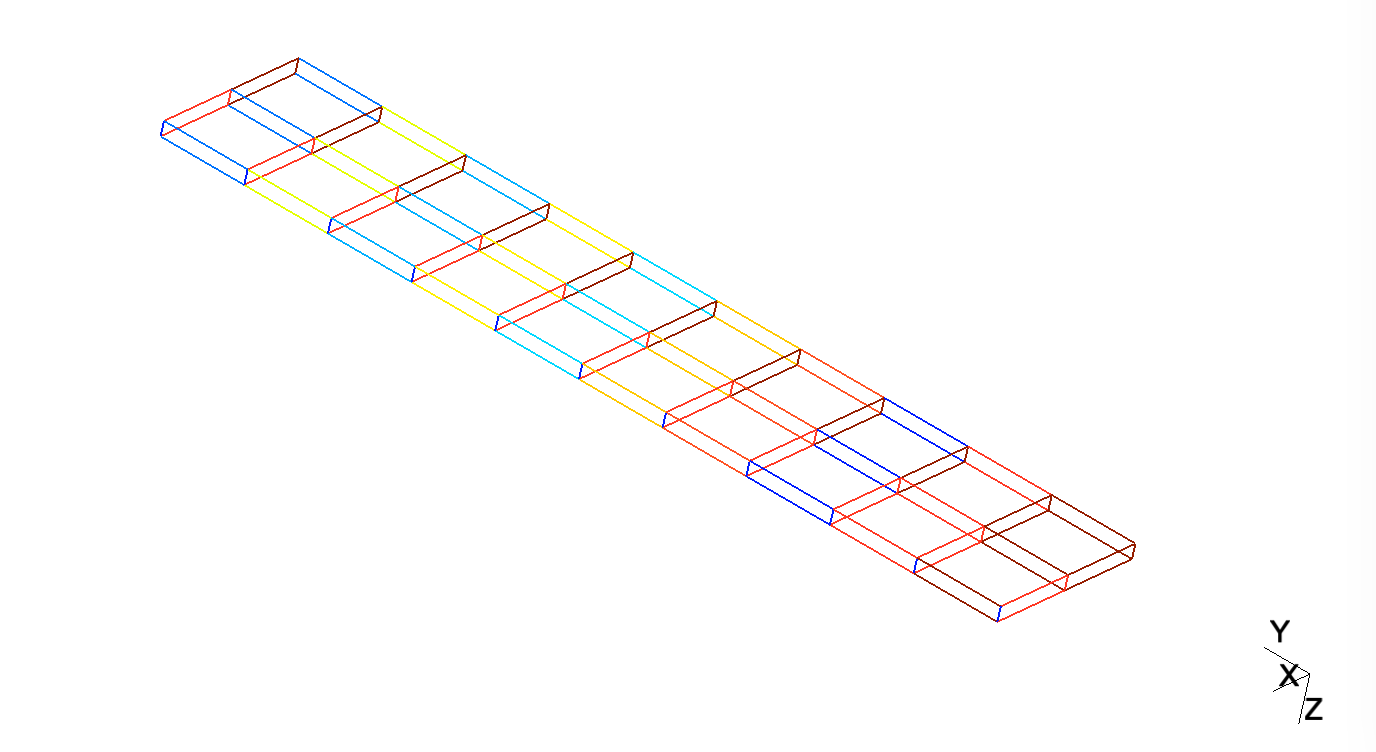
\includegraphics[width = 1\textwidth]{./Immagini/5_1.png}
	\caption{Initial FEM model for the Goland wing}
	\label{fig:5_1}
\end{figure}
For the aerodynamic mesh an airfoil are obtained using a 4\% thick parabolic arc, then the mesh is generated using 4 section until the wing span, for each section several point of the airfoil are considered, with a condensation of nodes on the trailing and leading edge, then the panel are obtained joining the nodes and the sections. In Fig. \ref{fig:5_2} is showed how the initial aerodynamic mesh is structured.
\begin{figure}[H]
\centering
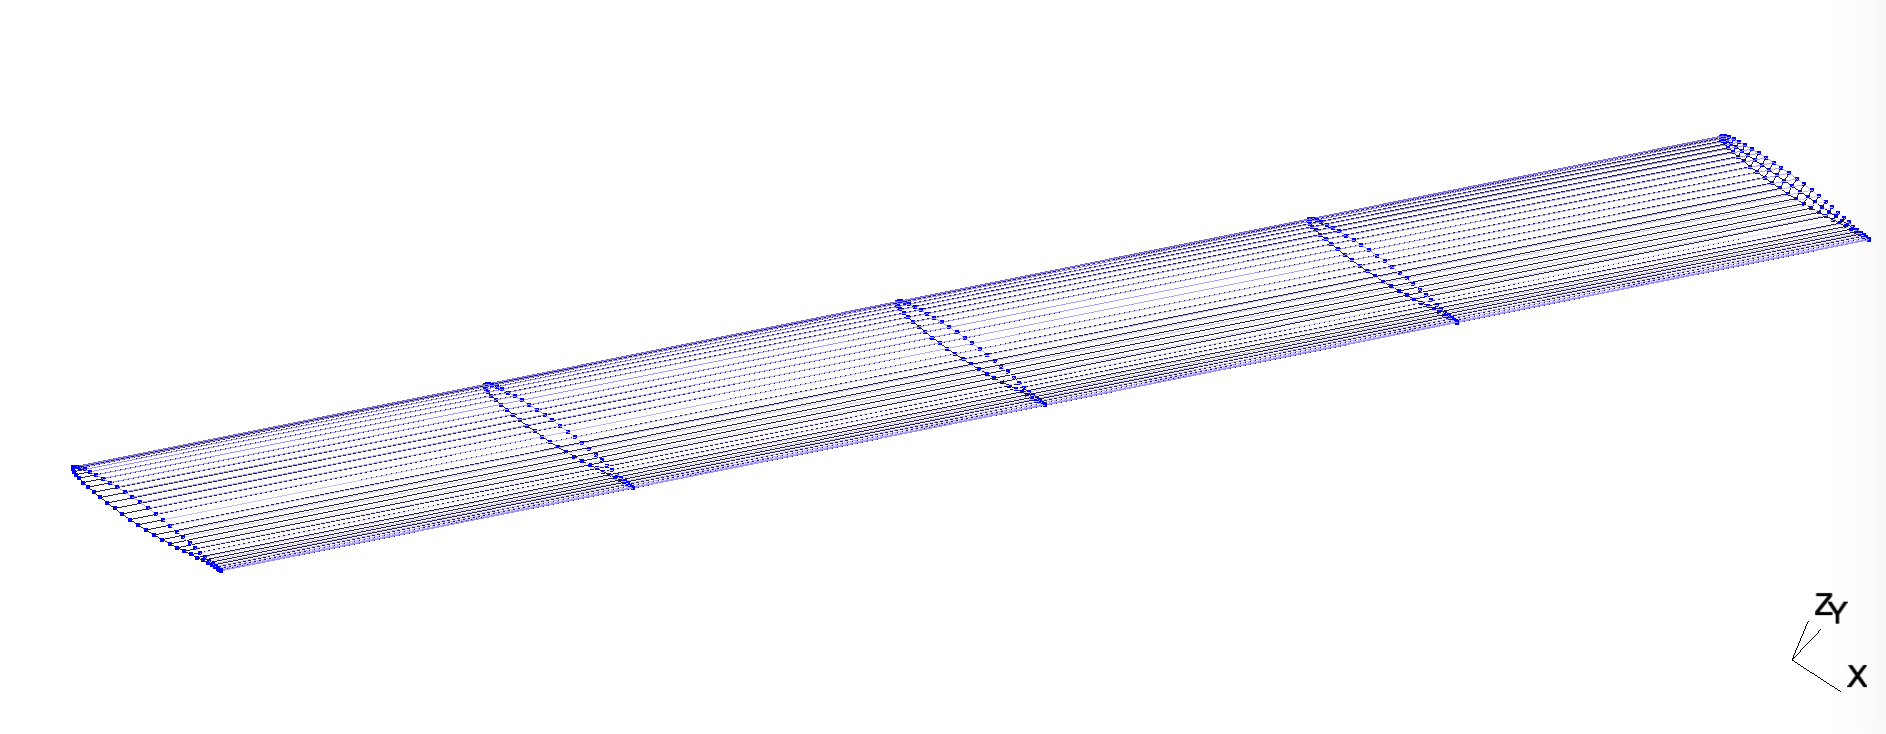
\includegraphics[width = 1\textwidth]{./Immagini/5_2.png}
\caption{Initial aerodynamic mesh for the Goland wing}
\label{fig:5_2}
\end{figure}

\section{CRM wing}
The second wing model used for the test cases is the NASA Common Research Model Wing \textbf{CRM}. This choice has been adopted in order to have a more complex wing's model, to access to more problematic and design's aspect, compared to the Goland wing, and the choice was the CRM, because several project is based on this model, so we can easily find in literature results to compare, and evaluate the quality of them.\\
The Common Research Model (CRM) consists of a contemporary supercritical transonic wing and a fuselage that is representative of a widebody commercial transport aircraft.  The CRM is designed for a cruise Mach number of $M_{\infty} = 0.85$ and a corresponding design lift coefficient of $C_L= 0.5$. \cite{nasa2}\\
The wing consist in a fullscale cantilevered wing. The CRM was generated as open geometry for the research, imagined for transport class aircraft with single-aisle configuration. The geometry of the wing is more complex of the Goland wing, in fact there are sweep angle, taper ratio, etc... .It's caraterized of a wing span of $58.76 \ m$, an aspect ratio of 9, a root cord of $7\ m$, a taper ratio of 0.275, a leading edge sweep angle of $35 \deg$, and a break along the trailing edge at 37\% of the semi-span, the wing reference area is $ 383.68\  m^2$. For the structure the wing box is defined to lie between 10\% and 70\% of the wing cord. 
\newpage
In Fig. \ref{fig:5_3} the plan view of the CRM wing is showed:
\begin{figure}[H]
	\centering
	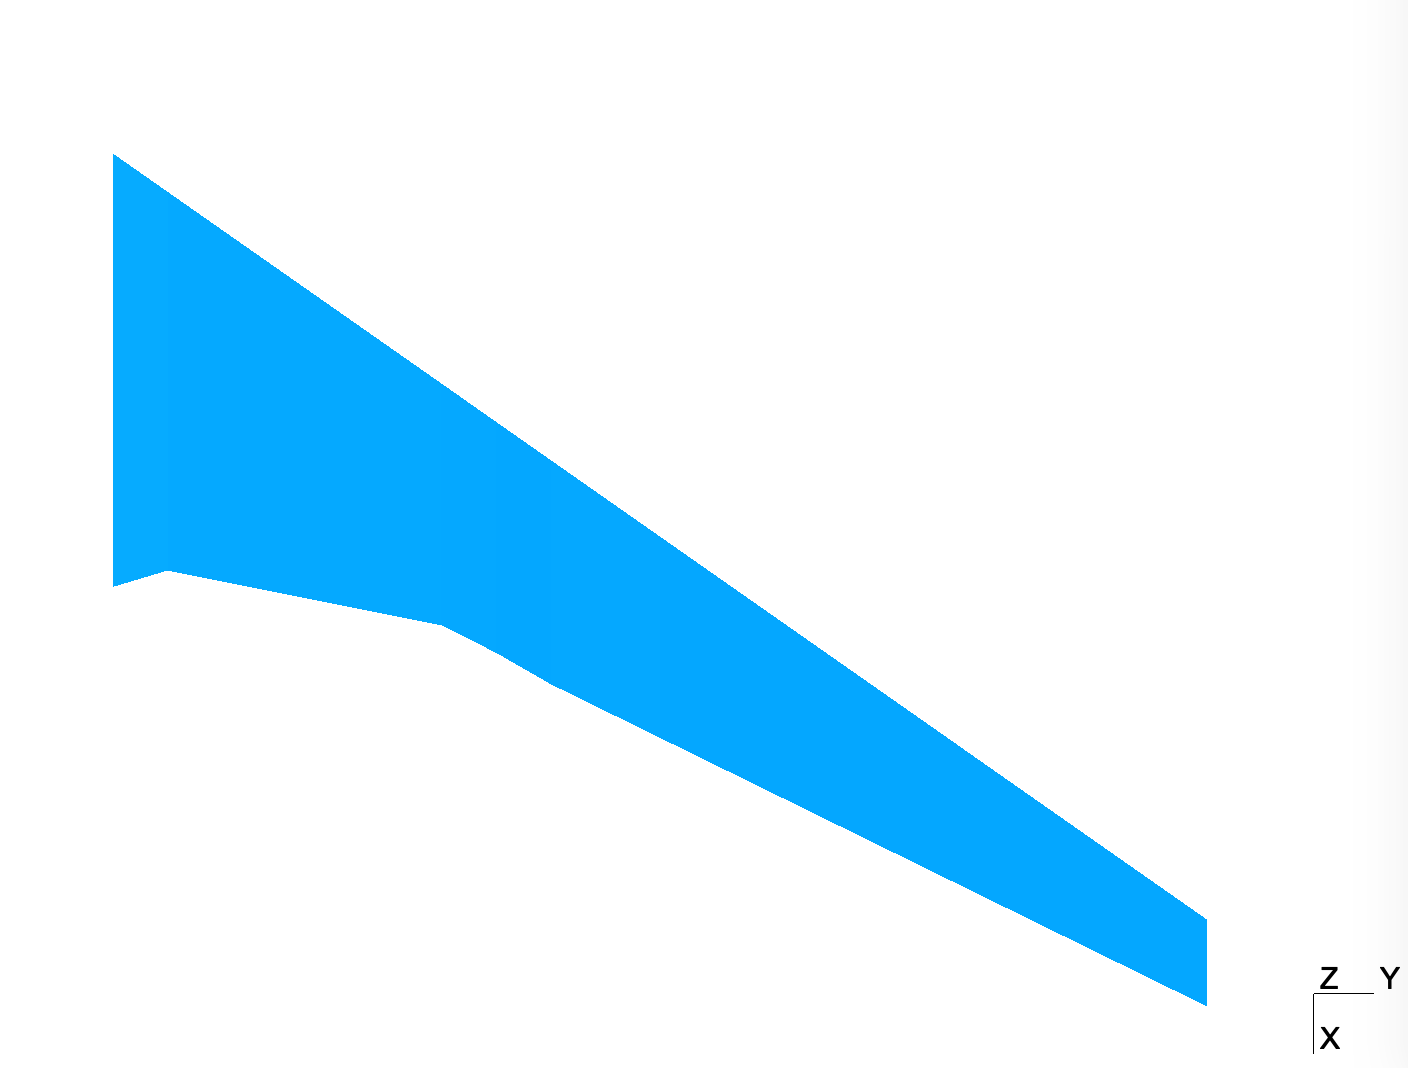
\includegraphics[width = 1\textwidth]{./Immagini/5_4.png}
	\caption{Plan view of the CRM wing geometry}
	\label{fig:5_3}
\end{figure}
For the structural model an high fidelity model have been created. All the component of the wing (ribs, spar, stringer, skin) are modeled using shell elements. Over 25'000 finite elements have been used. In Fig. \ref{fig:5_4} the complete FEM model is showed:
\begin{figure}[H]
	\centering
	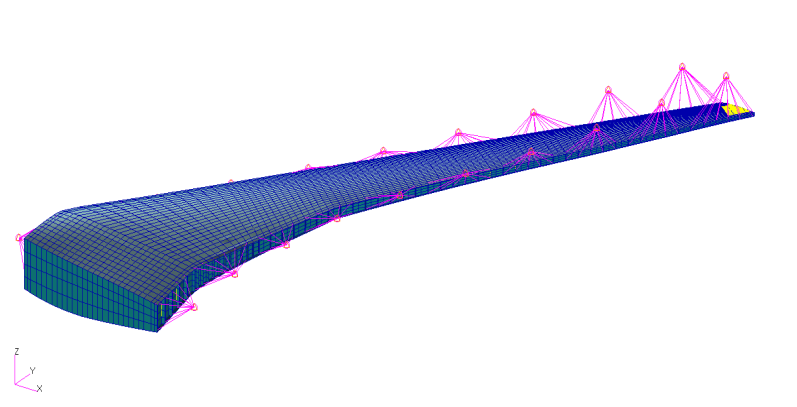
\includegraphics[width = 1\textwidth]{./Immagini/5_5.png}
	\caption{FEM model of CRM wing}
	\label{fig:5_4}
\end{figure}
The airfoil used to obtain the aerodynamic mesh is the CRM-65 in Fig. \ref{fig:5_5}, provided by NASA \cite{air}. The aerodynamic mesh is obtained using 50 different section, in order to take account of the taper ratio and the thickness. In Fig. \ref{fig:5_6} the aerodynamic mesh is showed:
\begin{figure}[H]
	\centering
	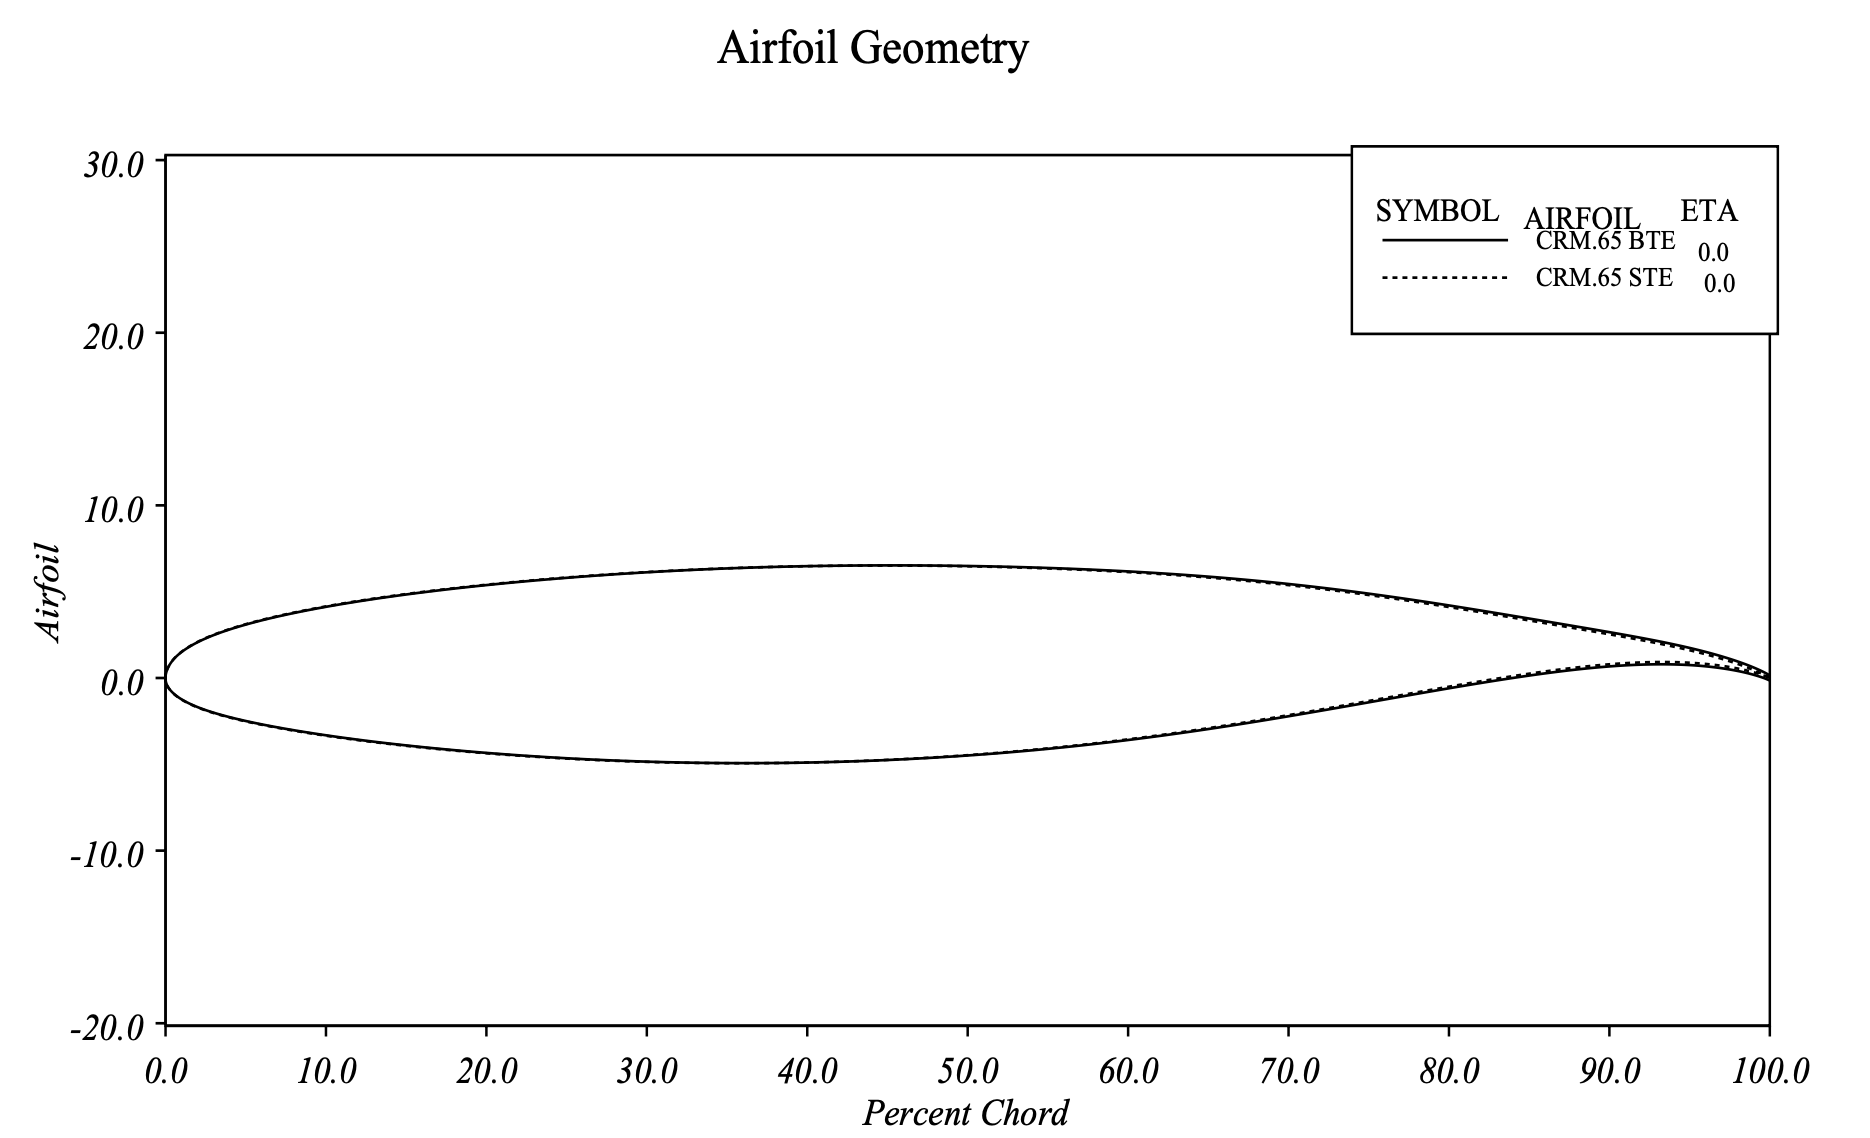
\includegraphics[width = 0.7\textwidth]{./Immagini/5_6.png}
	\caption{CRM-65 airfoil}
	\label{fig:5_5}
\end{figure}
\begin{figure}[H]
	\centering
	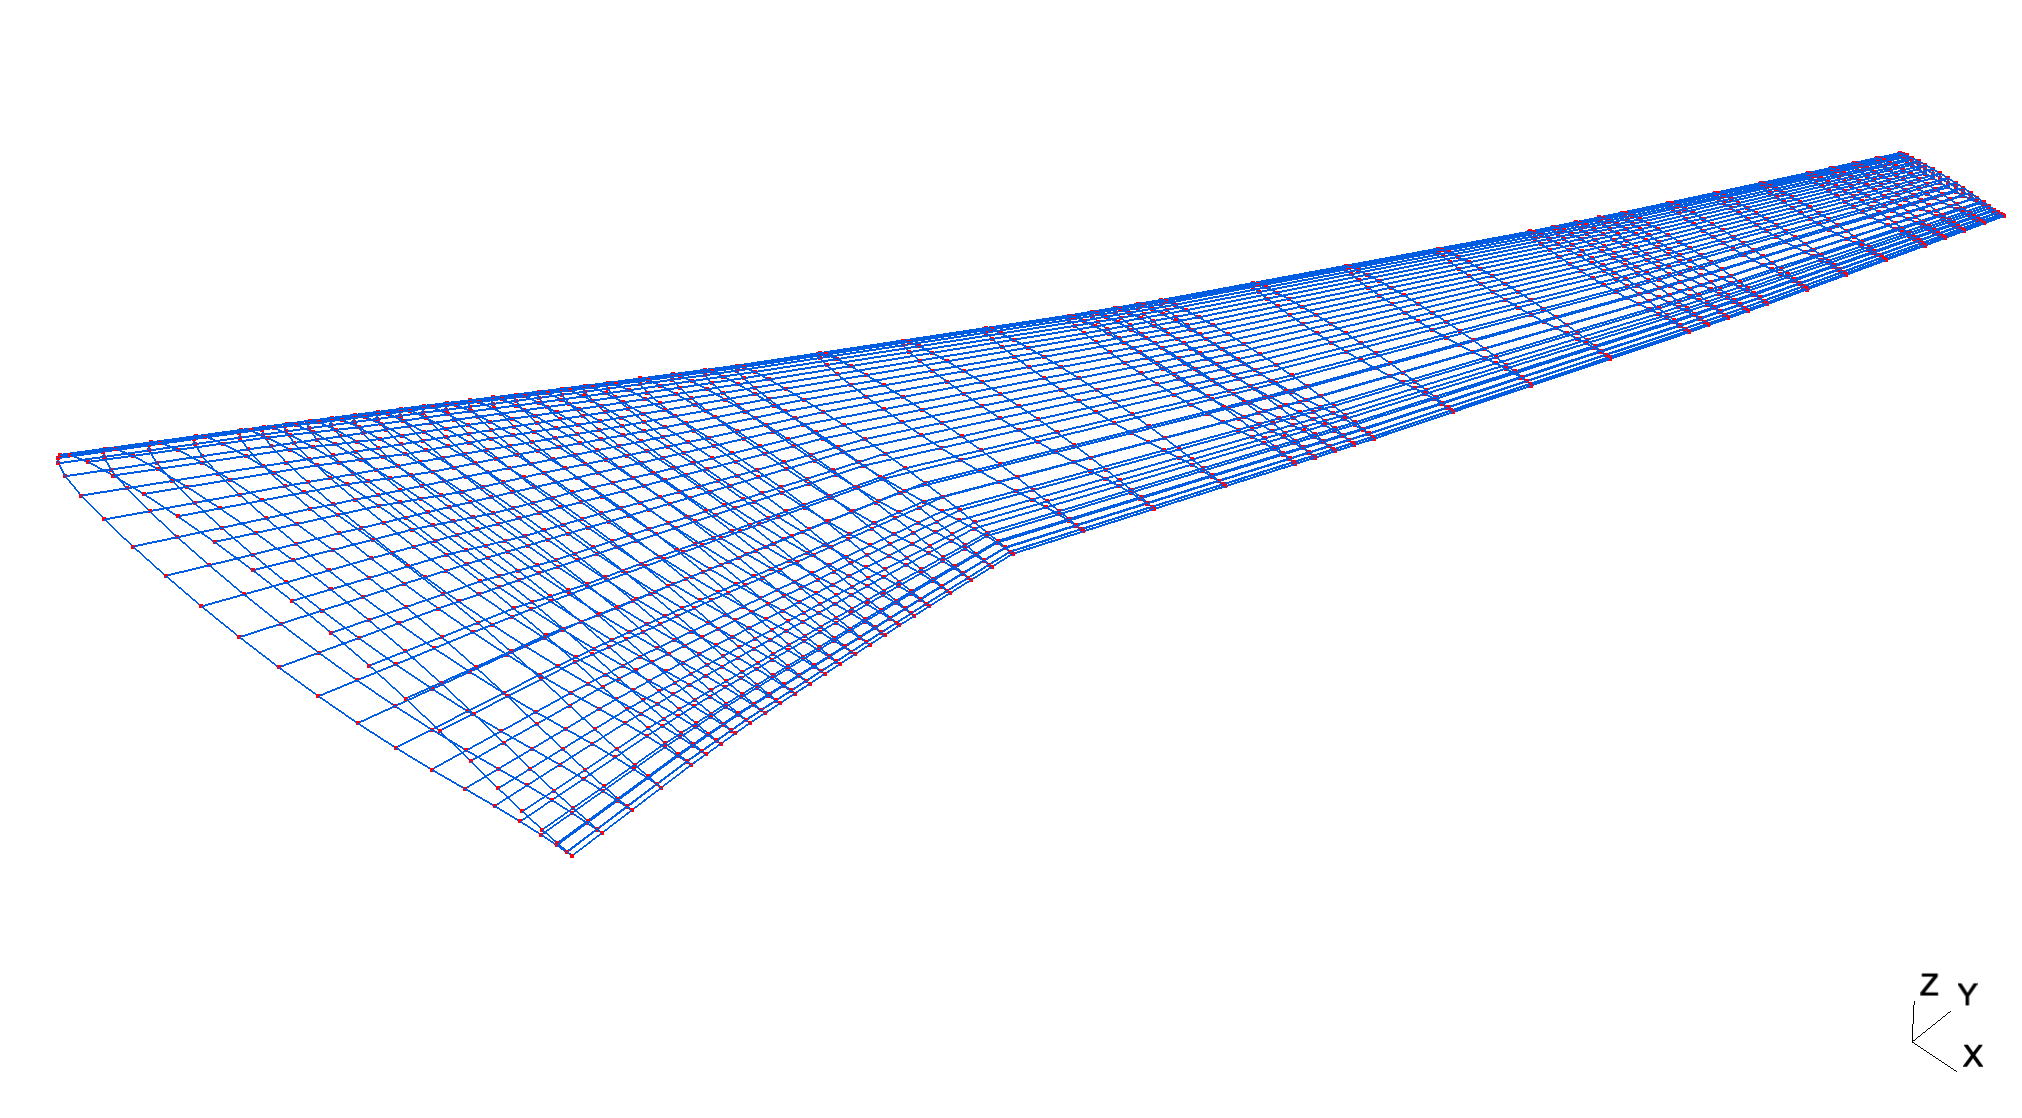
\includegraphics[width = 1\textwidth]{./Immagini/5_7.png}
	\caption{Aerodynamic mesh of the CRM wing}
	\label{fig:5_6}
\end{figure}
\section{CRM Wing Simple Model}
The CRM wing model allow to consider more parameters in the optimization process, but the cost of the structural and aerodynamic analysis for the model that we create are really high. In the test phase of the component, where coding or conceptual errors emerge, the time required to launch the code can be prohibitive. So to solve this problem a simple model of the CRM wing have been used, in order to have all the proprieties of the CRM wing but with a much less computation cost. The quality of the result is, of course, worse, but in that phases we wasn't interested to obtain result, but just to validate the code.\\
The most important changes are on the structural model. As first much less elements have been used, from 25'000 to 1'000, then instead to use shell elements for all the components, beam elements have been used for stringer and spars.\\
In Fig. \ref{fig:5_7} the structural mesh of the simple model of the CRM wing is showed, the beam elements are in red while the shell elements are in blue:
\begin{figure}[H]
	\centering
	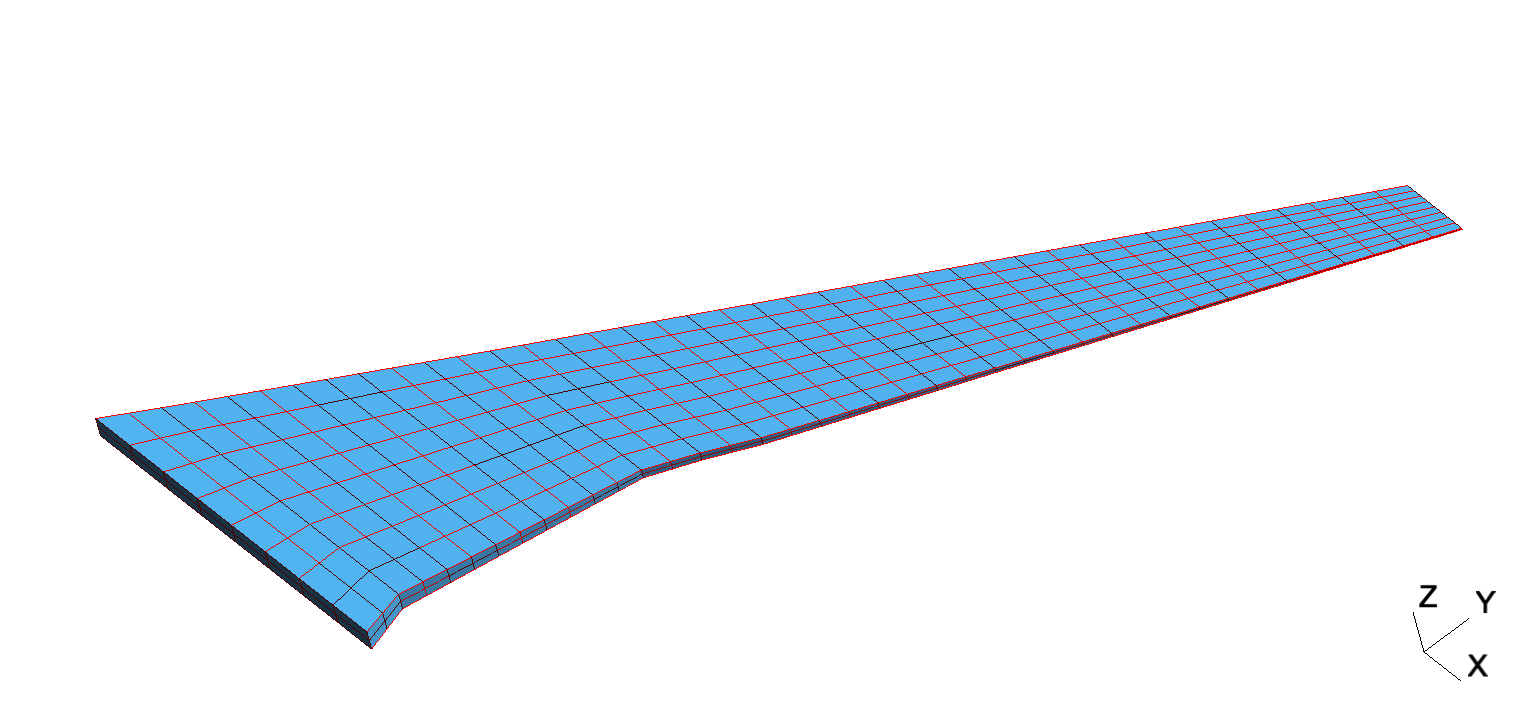
\includegraphics[width = 1\textwidth]{./Immagini/5_8.png}
	\caption{Aerodynamic mesh of the simple model CRM wing}
	\label{fig:5_7}
\end{figure}
Also the aerodynamic mesh is simple. In this case we just reduced the number of section, from 50 to 20. In Fig.\ref{fig:5_8} is showed the aerodynamic mesh of the simple CRM wing model:
\begin{figure}[H]
	\centering
	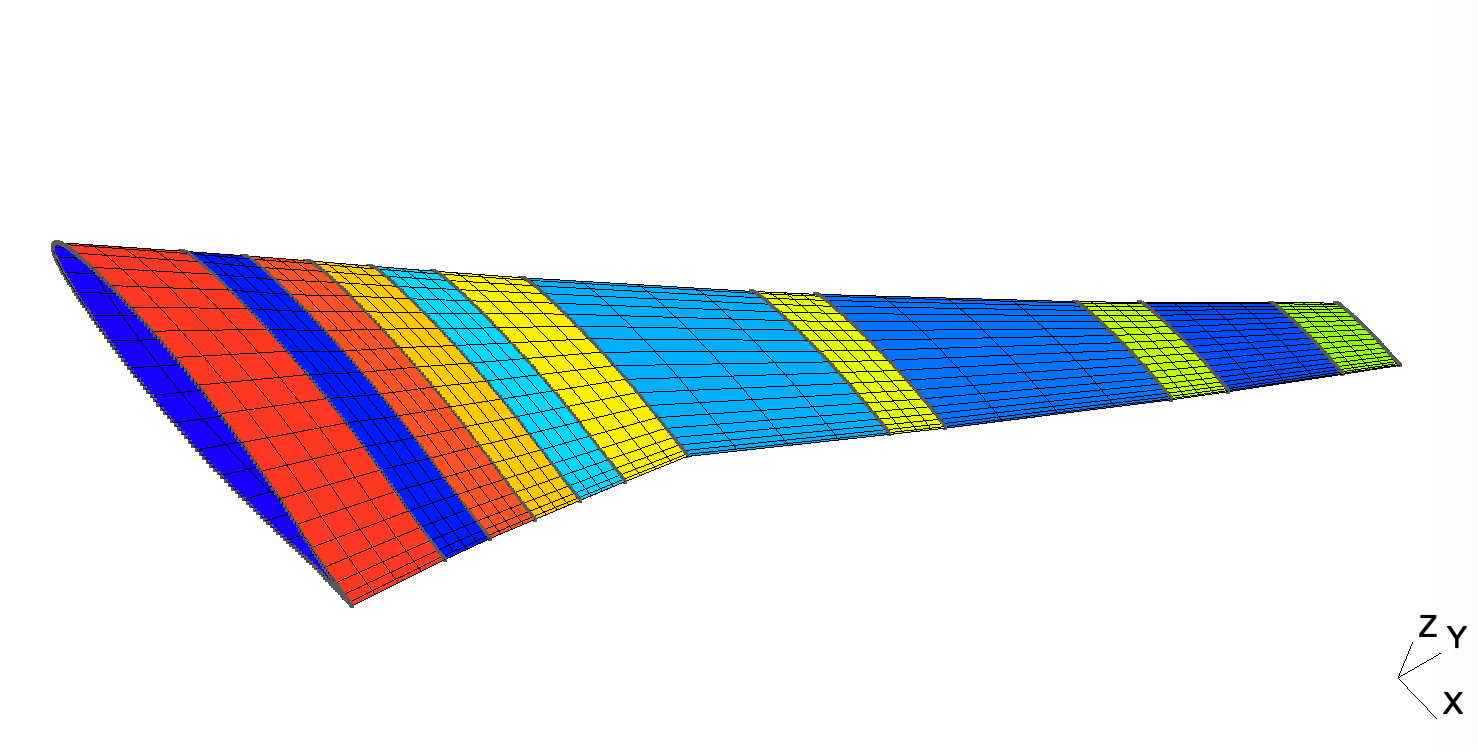
\includegraphics[width = 1\textwidth]{./Immagini/5_9.png}
	\caption{Aerodynamic mesh of the simple model CRM wing}
	\label{fig:5_8}
\end{figure}
\section{Different Options for the Optimization}
Several test cases have been performed in order to validate the different components, to test the different drivers, the different wing model. So each test case represent a combination of different option and has different goal. In Tab. \ref{tab:t4} there are collect all the possible option used in the various test case:
% Please add the following required packages to your document preamble:
% \usepackage{multirow}
% Please add the following required packages to your document preamble:
% \usepackage{multirow}
\begin{table}[H]
	\centering
	\begin{tabular}{c|c}
		\hline
		\textit{Options}                                                               & \textit{Possible Choice}            \\ \hline
		\multirow{3}{*}{Wing Model}                                                    & Goland Wing                         \\
		& CRM Wing                            \\
		& CRM Wing Simplified                 \\ \hline
		\multirow{2}{*}{Driver}                                                        & COBYLA                              \\
		& SLSQP                               \\ \hline
		\multirow{4}{*}{\begin{tabular}[c]{@{}c@{}}Design\\ Variables\end{tabular}}    & Angle of Attack $\alpha$            \\
		& Thickness of Shell Elements         \\
		& Sweep Angle $\Lambda$               \\
		&  Wingspan $b$                                   \\ \hline
		\multirow{3}{*}{\begin{tabular}[c]{@{}c@{}}Objective\\  Function\end{tabular}} & Mass $m$                            \\
		& Induced Drag Coefficient $C_{D_i}$  \\
		& Generic Function $f$                \\ \hline
		\multirow{3}{*}{\begin{tabular}[c]{@{}c@{}}Generic \\ Options\end{tabular}}    & Constraint Aggregation              \\
		& Design Varibles Limit as Constraint \\
		& Reduced Structural model            \\ \hline
	\end{tabular}
\caption{Different option selectable for the optimization}
\label{tab:t4}
\end{table}
\section{Problems}
During the test cases several problems emerge. In this section we will explain the most relevant problems, and the relative solution that we find. 
\subsection{Cobyla Design Variables Limits}
One of the first problem that have emerged when we pass to the CRM wing cases was relative to the use of the optimization driver COBYLA. The problem was that when the thickness of the wing tip shell elements, the zone of the wing characterized to the biggest value of displacements , start to be to little, the displacements start to being really impressive. Then this displacements are moving into the aerodynamic mesh using the interpolation. Now if the wing tip section nodes are moving too much, the aerodynamic analysis will fail, because the mesh assume a weird shape. That's cause the crash of the program and interrupts the optimization. The direct consequence is to set limits for the design variables, in this case limits on the minimum value of the shell elements thickness, in order to avoid that the displacements being huge. Then we set limits on the thickness as $10^{-3}\ m$.\\
Using the COBYLA optimization we see that, despite the design variables limits was exactly set, the optimization still crash. Then opening the database of the iterations we saw that the limits of the design variables are not respected, as we can see in Fig. \ref{fig:5_9}:
 \begin{figure}[H]
 	\centering
 	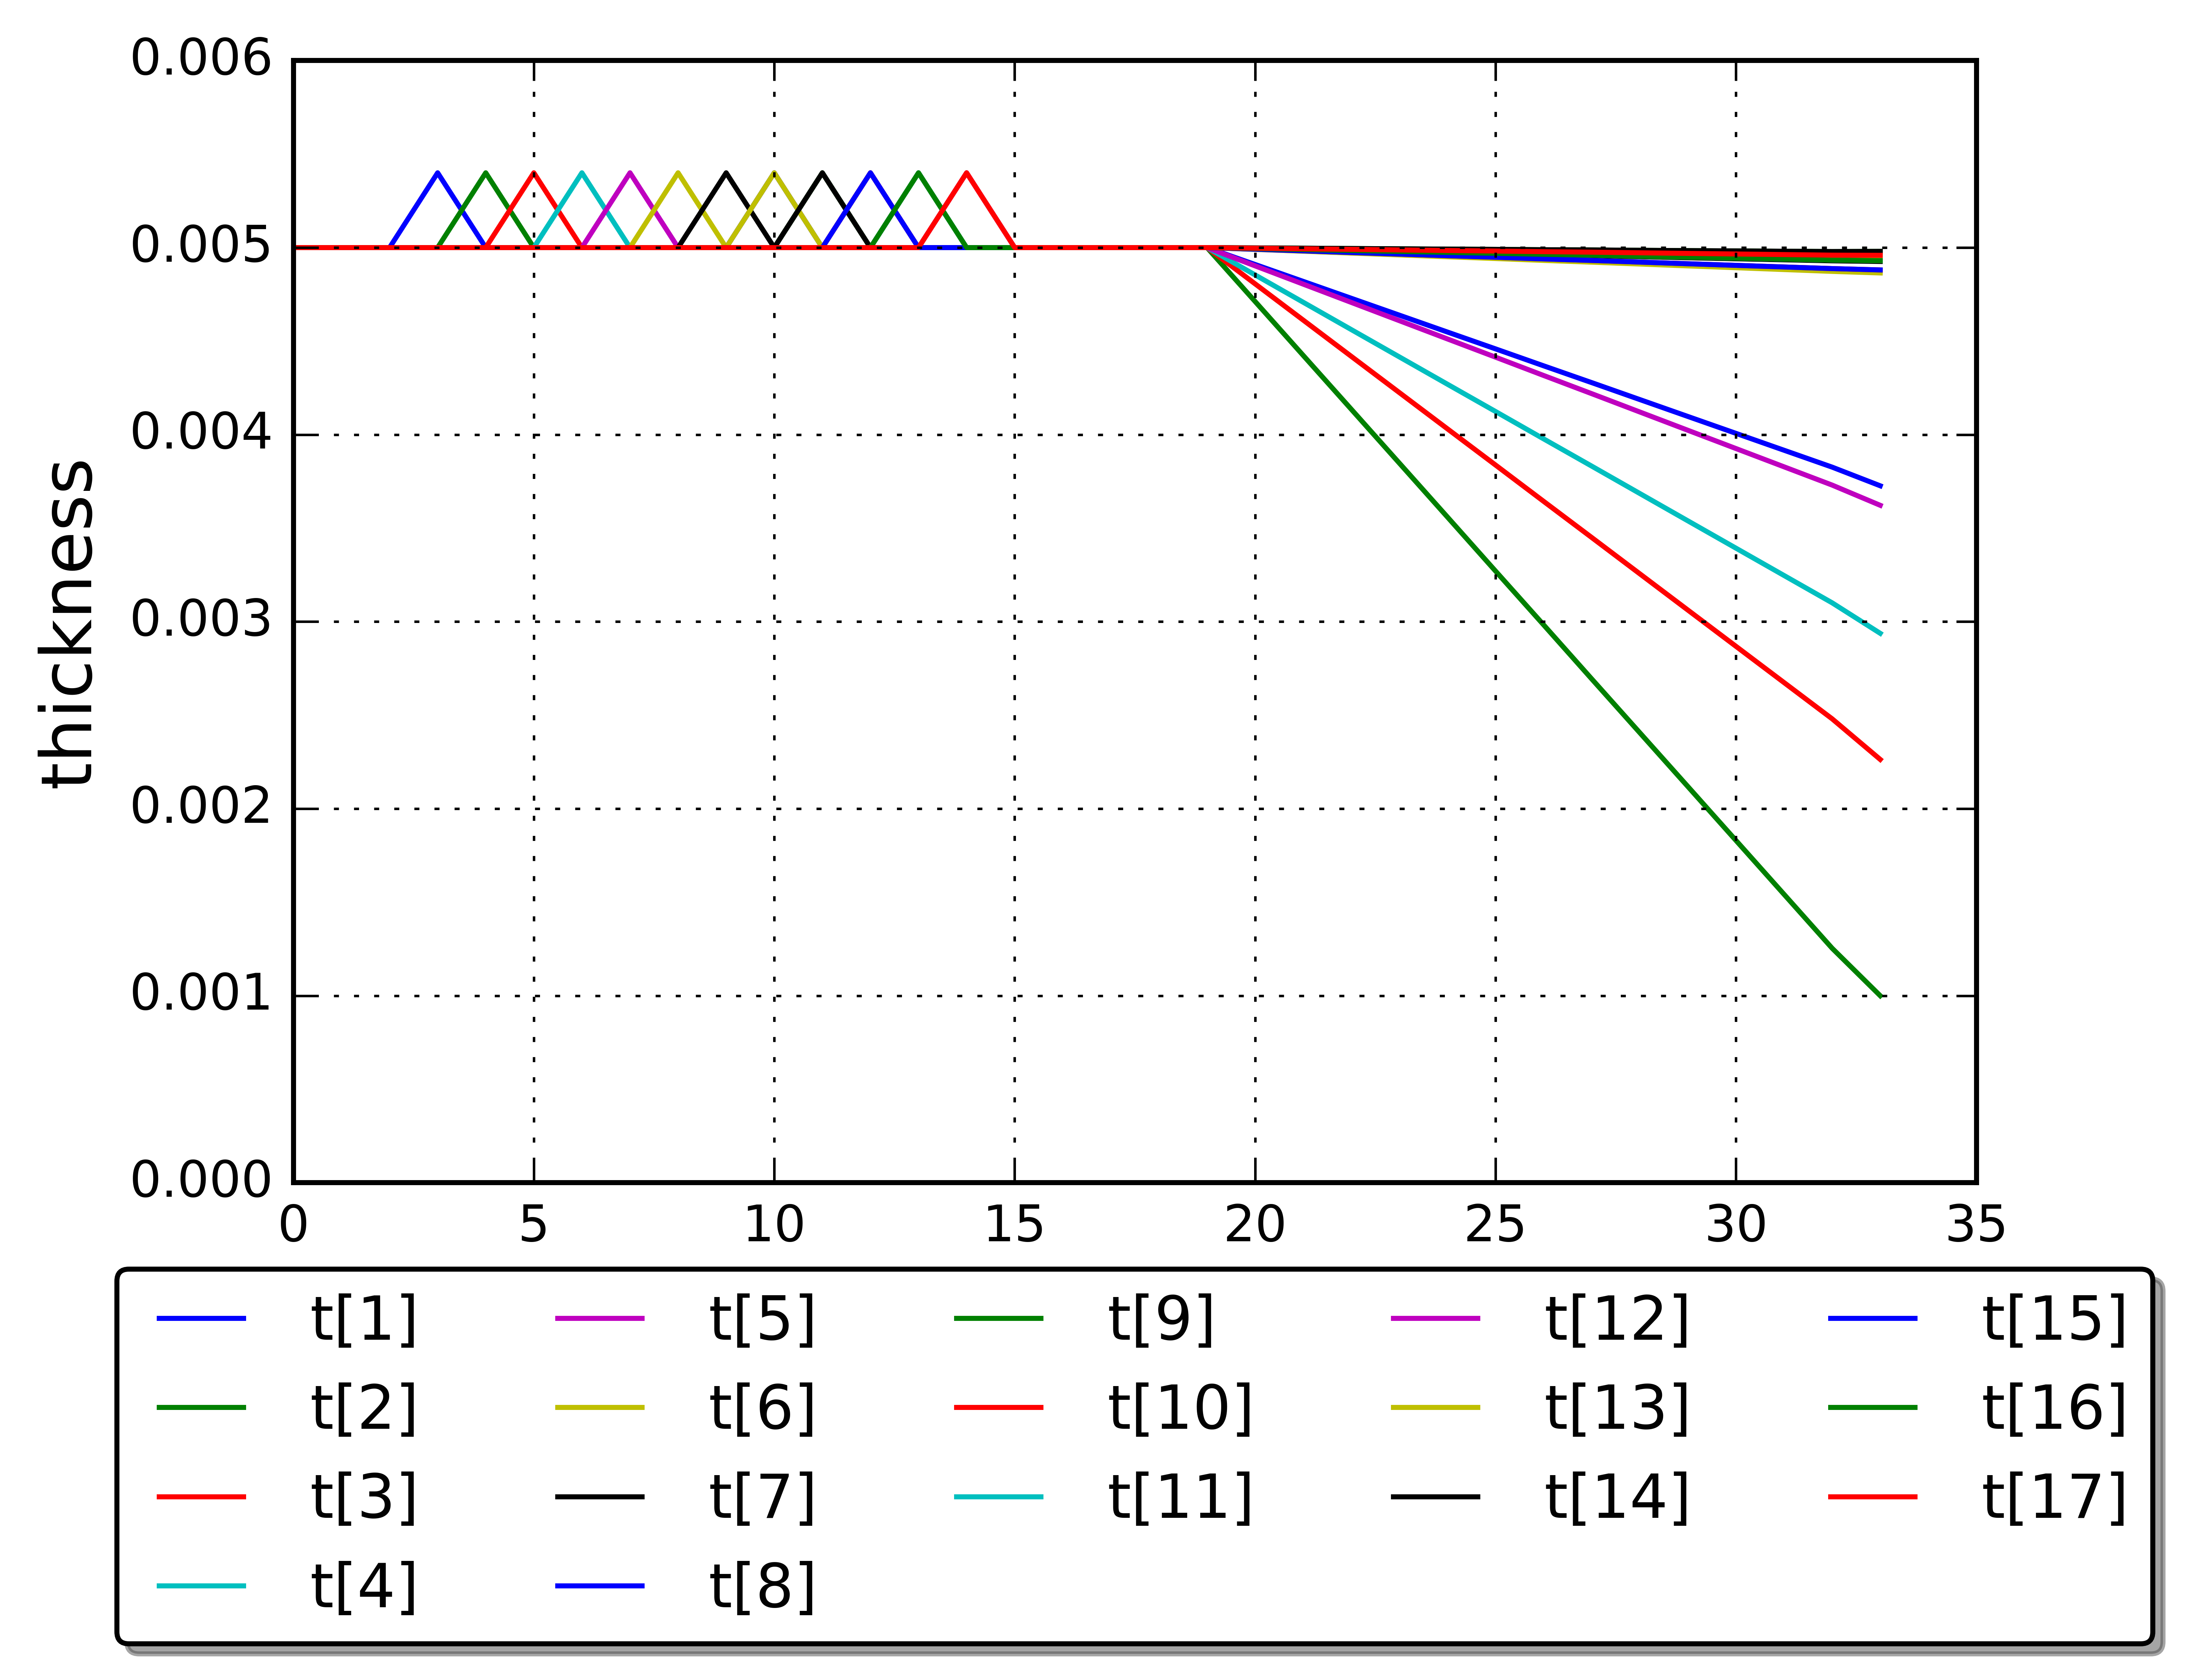
\includegraphics[width = 0.8\textwidth]{./Immagini/5_10.png}
 	\caption{Thickness variation in a COBYLA optimization}
 	\label{fig:5_9}
 \end{figure}
As we can see the optimization crashes at the iteration 34, because the thickness of the section 16 is lower than $10^{-3}\ m$. The problem is that COBYLA doens't respect the design variables limits. That's is result of the is a consequence of how it was programmed, COBYLA is a driver programmed to get results, so when it decide the direction of the optimization, in this case the direction is to reduce the thickness of section in order to obtain a reduction of the mass of the wing, it still work in order to get the convergence of the objective function respecting the constraints. \\
To solve this problem, and avoid the crashes, our solution was to set also the thickness limits of the section as constraint, in order to be respected by COBYLA. So a new set of constraint have been created, the constraints equation check for each iteration if the minimum value of the thickness is bigger than the limit which we set:
\begin{equation*}
con(t_i)=t_i-t_{i_{min}} >0 \qquad i=1,2,...,n_t
\end{equation*}
where $con(t_i)$ is the constraint function, $t_i$ the value of the thickness of the section $i$, $t_{i_{min}}$ the limit of the thickness and $n_t$ the number of the section with different thickness.\\
In order to check if the solution works, we start a particular optimization focused on the reduction of the thickness for all the section, and check if the limits on the thickness if finally respected, as is showed in Fig. \ref{fig:5_10}:
 \begin{figure}[H]
	\centering
	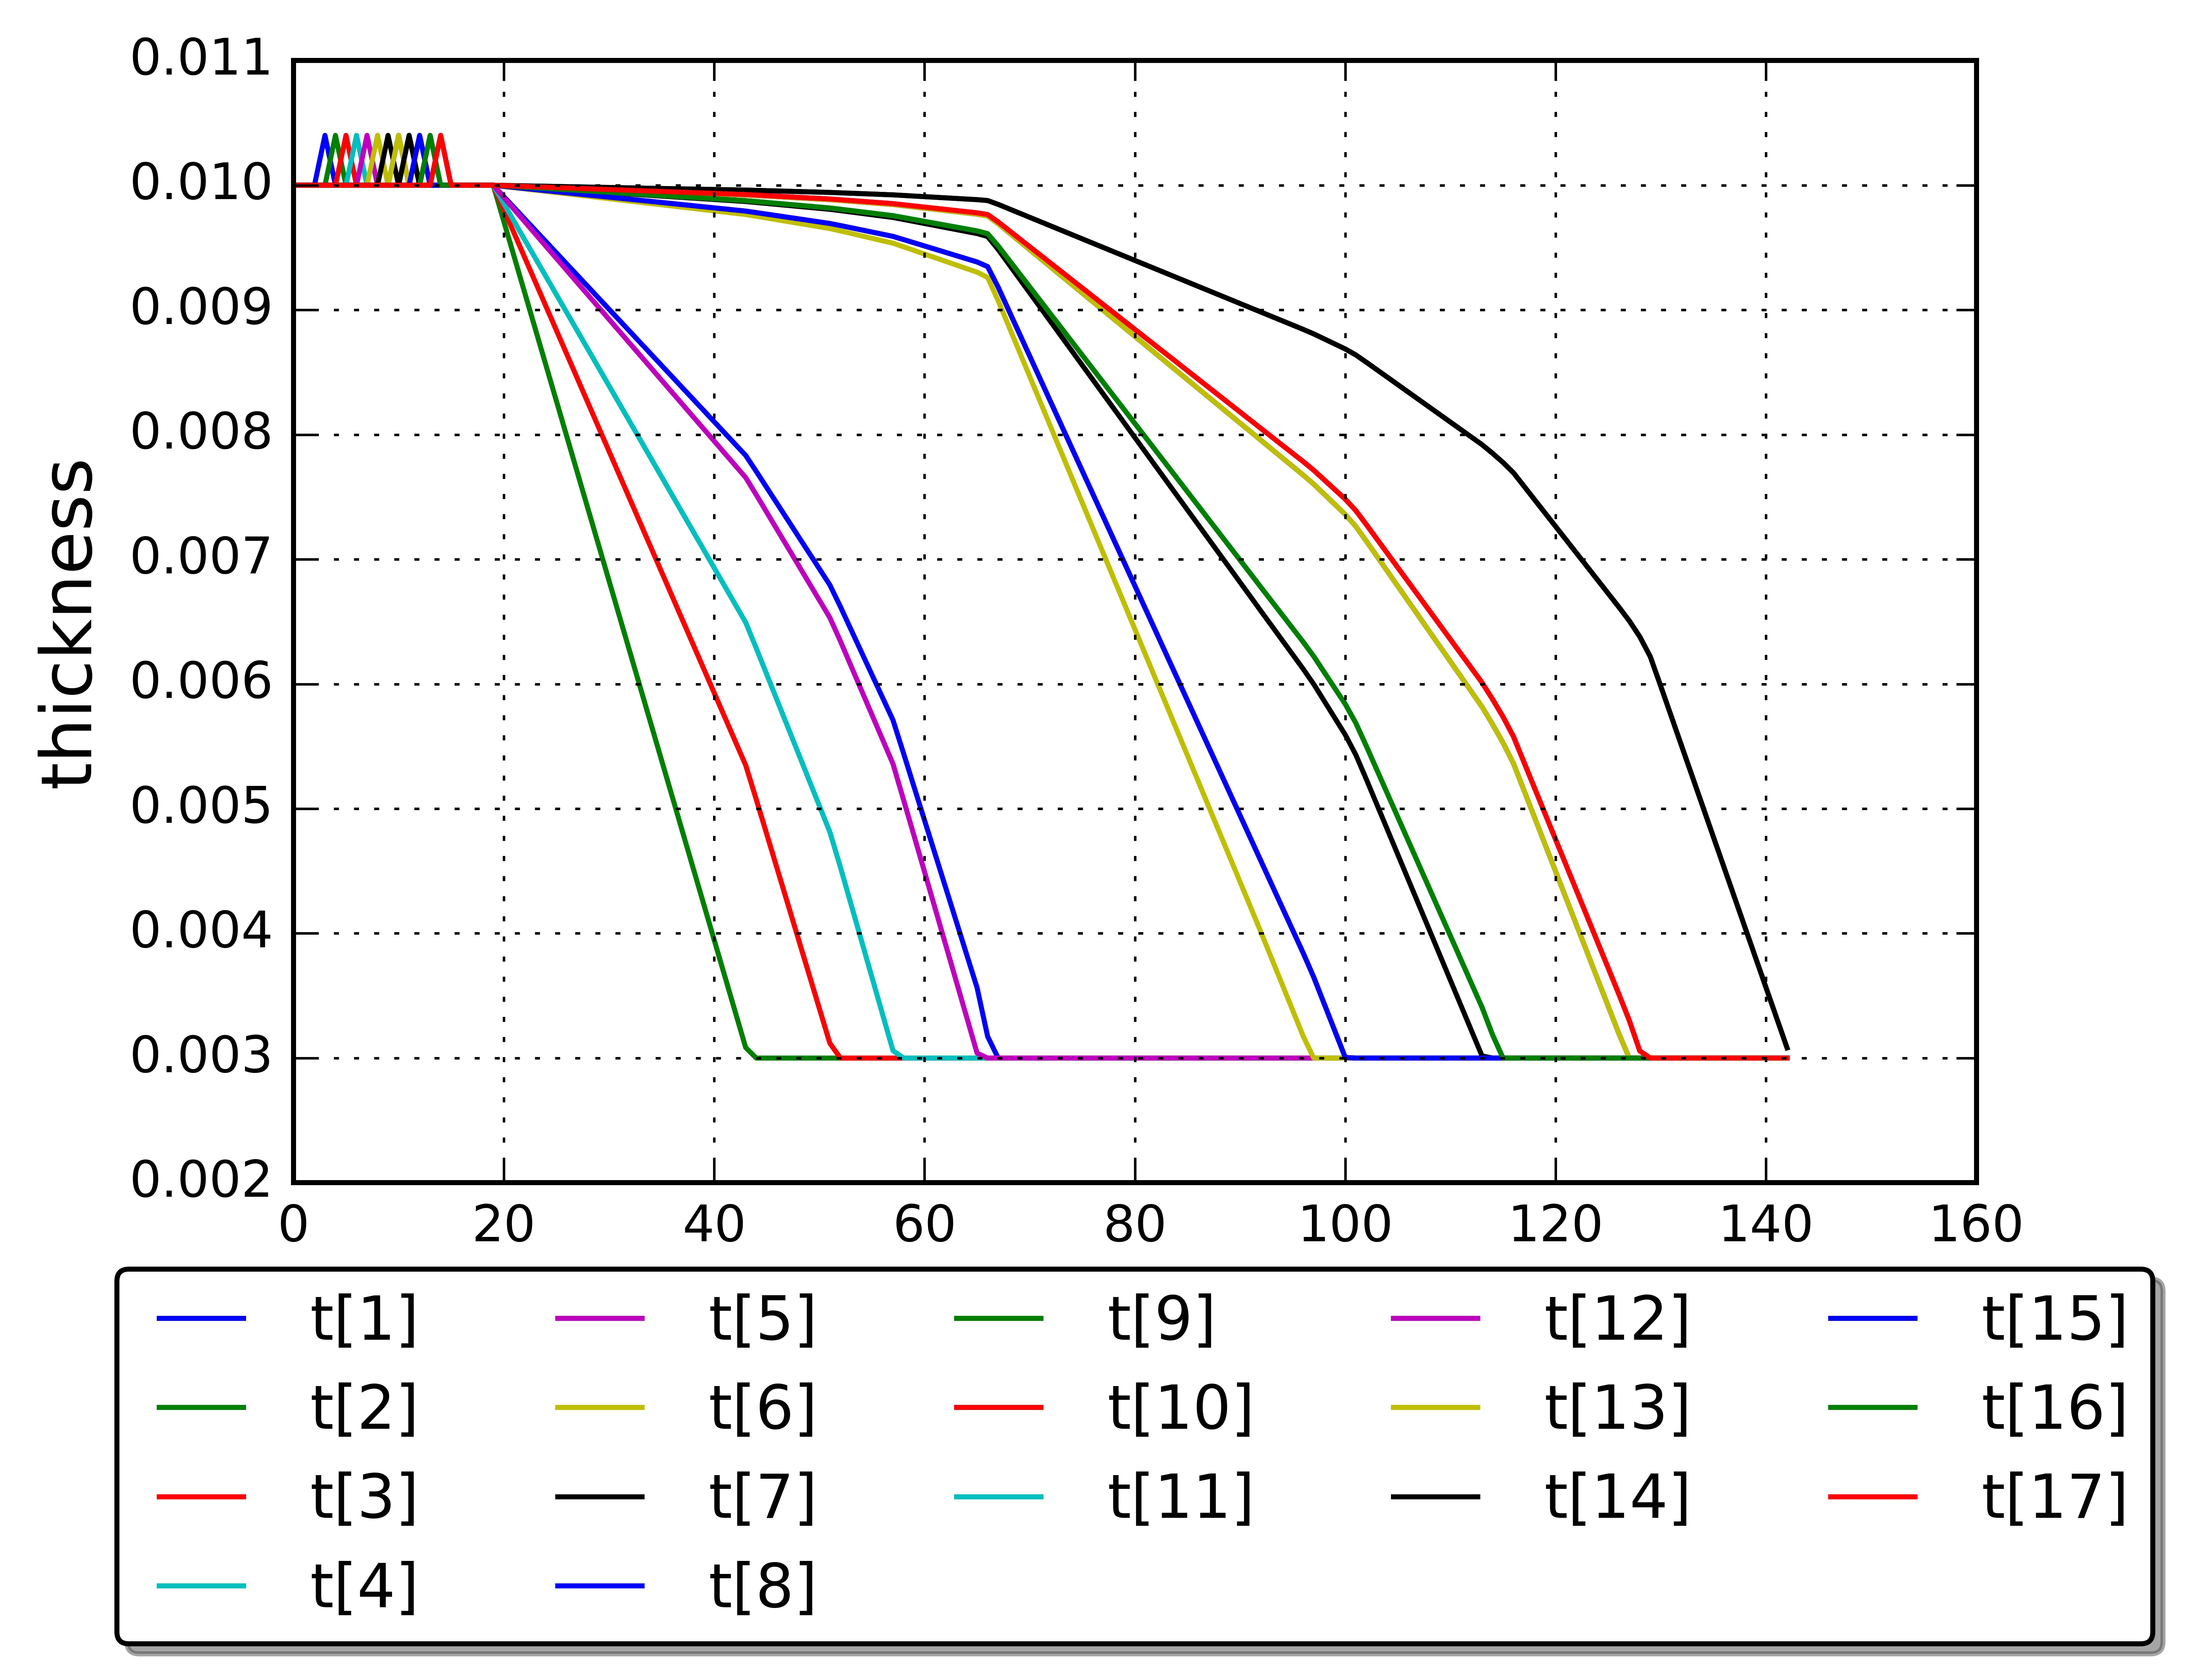
\includegraphics[width = 0.8\textwidth]{./Immagini/5_11.png}
	\caption{Thickness variation after design limits correction}
	\label{fig:5_10}
\end{figure}
As we can see the correction works well, in fact when the thickness reach the design limit, in this case $3*10^-3$, that value will not more changed, and the stability of the optimization is guaranteed.
\subsection{Finite Difference Gradient Evaluation Error }
Another error has emerged using the SLSQP driver. As we said in the chapter 2, to evaluate the gradient, for the gradient based optimization using SLSQP, we use the finite difference method. In our specific case one of the gradient that we need for the optimization, being the thickness of the section a design variables, and the Von Mises stress a constraint, like the lift, and the mass an objective, the gradient of these function respect to the thickness.\\
As we explain the structural analysis and the aerodynamic analysis is performed by the external codes, respectively NASTRA95 and Panair. So to compute the gradient the flow-chart is the following, for example in the case of the gradient of the mass respect the thickness:
\begin{enumerate}
	\item Set the the starting value of the thickness
	\item Perform an static structural analysis
	\item Extract from the output file the value of the mass
	\item Change the thickness of the finite difference step
	\item Perform an static structural analysis
	\item Extract the new value of the mass from the output file
	\item Compute the gradient using the finite difference equation
\end{enumerate}
The problem that we found was that using the default settings, the solver can't evaluate the gradient, as the mass didn't change after a change of the thickness. That happens because NASTRAN95 use a 8 bit floating point numeration; so the finite difference step set as default for SLSQP is $10^-4$, so the effect that the variation of this step induce on the structural mass is really little, and it changes just the 9th or 10th significant digits, then NASTRAN95 cut the information after the 8th significant digit, so he will lose the information on the variation of the mass, and the mass seems unchanged.\\
To solve this problem is just necessary to specify in the setting of the driver the new step used for the finite difference, in order to induce a bigger variation on the structural mass, then the information on the variotion of the mass will not lose, in our case a step of $10^-2$ it's enough to compute correctly the gradient.
\subsection{Nastran Output File Reader}
Another problem emerged in the test cases is relative to the structural component, specifically for the output file reading method. In order to extract the information of the Von Mises stress for each element we set NASTRAN95 to save this information in a \textit{.pnh} file, characterized by a special structure of the file. Then the structural component after the analysis access to this output file, and an algorithm have been written to associate all the stress to the elements and save these information in a python dictionary. The algorithm have been written in relation at the output file of an analysis performed on the CRM wing, where only shell elements have been used. In the moment that we introduce the simple CRM wing model that contains also beam elements, the structure of the output file changes, then the algorithm can't read successfully it. In the first moment a new algorithm have been written to read correctly also the new output file, but we are working in order to make it universally. The idea is to use an \textit{.exe} file that convert the \textit{.pnh} file. The difference between the output files is that the number of the stresses depends on the number of the degree of freedom of the elements, then the data is collected on more lines. The \textit{.exe} file is structured to convert the file in a file where all the stress of one element are collected on just one line, then is easy to write an algorithm to collect the data independently of the wing structural model chosen. 
